\chapter{Neoclassical Growth vs.\ Data}

The preceding chapters developed the neoclassical growth framework---from the Solow model to its recursive formulation in the Ramsey--Cass--Koopmans model, together with computational tools such as Value Function Iteration. We now confront the theory with cross-country data. The central question is: does the model's signature prediction of convergence actually hold? If not, what modifications can reconcile theory with evidence?

\section{The Convergence Puzzle}

A central prediction of the Solow model is \textit{unconditional convergence}: because the marginal product of capital is high when capital is scarce, poorer countries should grow faster than richer ones and eventually catch up. Formally, under globally diminishing returns, the capital accumulation equation
\[
k_{t+1} = sf(k_t) + (1-\delta)k_t
\]
is a strictly concave function of $k_t$, crossing the 45-degree line exactly once at a unique, globally stable steady state $k^*$. Regardless of the initial capital stock $k_0 > 0$, the economy eventually converges to $k^*$.

The cross-country data, however, paint a considerably more complicated picture. The diagrams below illustrate, in stylized form, the joint distribution of initial income and subsequent growth rates across two historical periods.

\begin{center}
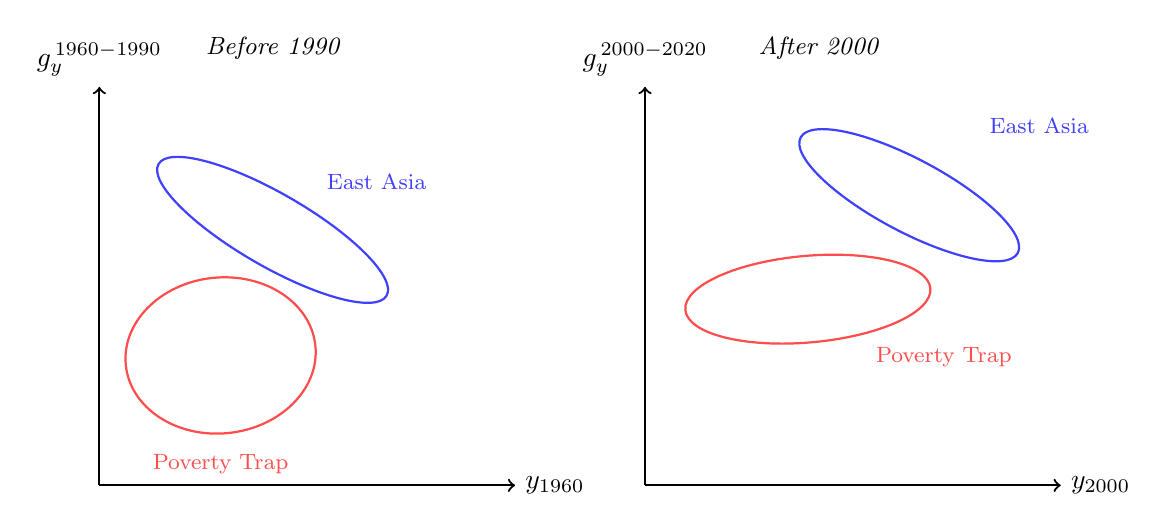
\begin{tikzpicture}[scale=1.1]

%% LEFT PANEL: Before 1990
%% Both clusters at similar low x (similar y_1960).
%% East Asia: upper, thin, tilted upward.
%% Poverty trap: lower, large and ROUND/TALL -- high dispersion in g_y.
\begin{scope}[xshift=0cm]
    \draw[->, thick] (0,0) -- (4.8,0) node[right] {$y_{1960}$};
    \draw[->, thick] (0,0) -- (0,4.6) node[above] {$g_y^{\,1960\text{-}1990}$};
    \node[font=\itshape\small] at (2.0, 5.05) {Before 1990};

    % East Asia: thin, elongated, tilted ~+30 degrees, upper area, near low x
    \draw[thick, blue!75, rotate around={-30:(2.0, 2.95)}]
        (2.0, 2.95) ellipse (1.52 and 0.42);
    \node[blue!75, font=\footnotesize] at (3.2, 3.5) {East Asia};

    % Poverty trap: BIG, nearly circular (tall minor axis = large g_y spread),
    % lower position, overlapping the lower-left part of East Asia ellipse
    \draw[thick, red!70, rotate around={6:(1.40, 1.50)}]
        (1.40, 1.50) ellipse (1.10 and 0.90);
    \node[red!70, font=\footnotesize] at (1.40, 0.25) {Poverty Trap};
\end{scope}

%% RIGHT PANEL: After 2000
%% East Asia has moved UPPER RIGHT (richer by 2000, still growing).
%% Poverty trap: still LOW x (still poor), but now FLAT -- dispersion has shrunk.
\begin{scope}[xshift=6.3cm]
    \draw[->, thick] (0,0) -- (4.8,0) node[right] {$y_{2000}$};
    \draw[->, thick] (0,0) -- (0,4.6) node[above] {$g_y^{\,2000\text{-}2020}$};
    \node[font=\itshape\small] at (2.0, 5.05) {After 2000};

    % East Asia: moved to upper right, thin, slight negative tilt
    % (internal convergence within the group)
    \draw[thick, blue!75, rotate around={-28:(3.05, 3.35)}]
        (3.05, 3.35) ellipse (1.42 and 0.42);
    \node[blue!75, font=\footnotesize] at (4.55, 4.15) {East Asia};

    % Poverty trap: FLAT/WIDE (small minor axis = small g_y spread),
    % still on the LEFT (still low income), overlaps lower-left of East Asia
    \draw[thick, red!70, rotate around={5:(1.88, 2.15)}]
        (1.88, 2.15) ellipse (1.42 and 0.50);
    \node[red!70, font=\footnotesize] at (3.45, 1.48) {Poverty Trap};
\end{scope}

\end{tikzpicture}
\end{center}

Two features of the data stand out. First, prior to 1990, the cross-country distribution of (initial income, growth rate) pairs is strikingly \textit{bimodal}. A cluster of East Asian economies---South Korea, Taiwan, Singapore, Hong Kong---achieved rapid catch-up growth of precisely the kind the Solow model predicts, growing fast from a moderate initial base. Yet a much larger cluster of low-income economies, concentrated in sub-Saharan Africa and parts of South Asia, exhibited persistently low or near-zero growth rates. These economies did not converge; they appeared stuck.

Second, and more troublingly, the bifurcation persists after 2000. The economies that were poor in 1960 and failed to grow remained poor in 2000, and their growth performance continued to lag. This pattern is what we call a \textit{poverty trap}: an apparently self-reinforcing state in which low income begets low investment, which begets low income.

The poverty trap constitutes a direct challenge to the basic neoclassical framework. Under globally diminishing returns, there is no reason for any economy with positive capital to stagnate indefinitely; every capital-scarce economy should enjoy high marginal returns and grow. To rationalize the data, we need to enrich the theory. We consider two distinct theoretical mechanisms.

\section{Two Mechanisms for Poverty Traps}

\subsection{Mechanism I: Non-Convexities and Multiple Steady States}

The first approach preserves the neoclassical structure but relaxes the assumption of globally diminishing returns. If returns to capital are \textit{locally increasing} over some intermediate range---due, for example, to fixed costs of technology adoption, learning-by-doing externalities, or coordination failures across sectors---the law of motion for capital becomes \textit{S-shaped} rather than globally concave.

The intuition is as follows. At very low capital levels, the economy cannot generate enough surplus to invest in the technologies and complementary inputs needed for growth: returns are low, investment is low, and the economy stagnates. But once capital crosses a critical threshold, positive externalities and complementarities kick in, and growth accelerates. Eventually, at high capital levels, the usual diminishing returns reassert themselves, and the economy settles into a high steady state.

Formally, the resulting law of motion $k_{t+1} = g(k_t)$ crosses the 45-degree line \textit{three times}, yielding multiple steady states:

\begin{center}
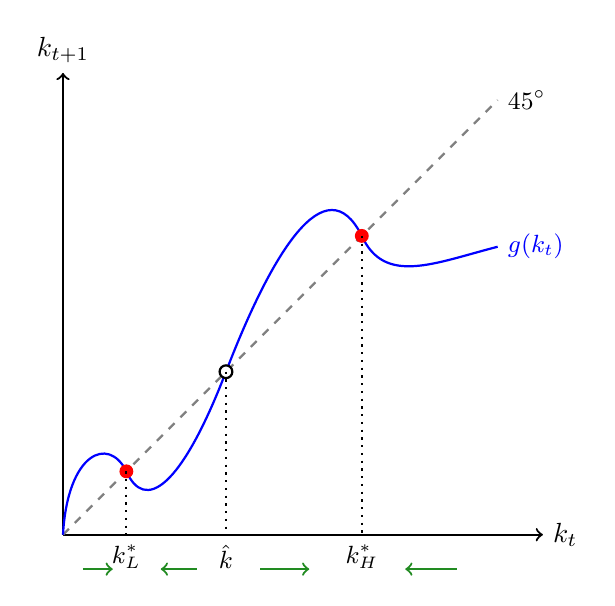
\begin{tikzpicture}[scale=1.15]
    % Axes
    \draw[->, thick] (0,0) -- (5.3,0) node[right] {$k_t$};
    \draw[->, thick] (0,0) -- (0,5.1) node[above] {$k_{t+1}$};

    % 45-degree line
    \draw[dashed, thick, gray] (0,0) -- (4.8,4.8)
        node[right, black, font=\small] {$45^\circ$};

    % S-shaped law of motion (Bezier, checked for monotonicity and sign of g(k)-k)
    \draw[thick, blue] (0,0)
        .. controls (0.05, 0.90) and (0.50, 1.10) .. (0.70, 0.70)
        .. controls (0.90, 0.25) and (1.30, 0.50) .. (1.80, 1.80)
        .. controls (2.30, 3.10) and (2.90, 4.10) .. (3.30, 3.30)
        .. controls (3.55, 2.75) and (4.10, 3.00) .. (4.80, 3.18)
        node[right, font=\small] {$g(k_t)$};

    % Steady states: filled circles = stable, open circle = unstable
    \filldraw[red] (0.70, 0.70) circle (2pt);
    \draw[thick, black, fill=white] (1.80, 1.80) circle (2pt);
    \filldraw[red] (3.30, 3.30) circle (2pt);

    % Dotted projections to x-axis
    \draw[dotted, thick] (0.70, 0.70) -- (0.70, 0)
        node[below, font=\small] {$k_L^*$};
    \draw[dotted, thick] (1.80, 1.80) -- (1.80, 0)
        node[below, font=\small] {$\hat{k}$};
    \draw[dotted, thick] (3.30, 3.30) -- (3.30, 0)
        node[below, font=\small] {$k_H^*$};

    % Direction-of-motion arrows beneath the x-axis
    % k < k_L*: g(k) > k, capital rises (rightward)
    \draw[->, thick, ForestGreen] (0.22, -0.38) -- (0.55, -0.38);
    % k_L* < k < hat{k}: g(k) < k, capital falls (leftward)
    \draw[->, thick, ForestGreen] (1.48, -0.38) -- (1.08, -0.38);
    % hat{k} < k < k_H*: g(k) > k, capital rises (rightward)
    \draw[->, thick, ForestGreen] (2.18, -0.38) -- (2.72, -0.38);
    % k > k_H*: g(k) < k, capital falls (leftward)
    \draw[->, thick, ForestGreen] (4.35, -0.38) -- (3.78, -0.38);
\end{tikzpicture}
\end{center}

The three intersections yield two stable and one unstable steady state:

\begin{itemize}
    \item $k_L^*$: the \textbf{low stable steady state}---the poverty trap. For any initial capital $k_0 < \hat{k}$, the economy converges to $k_L^*$. The low steady state is stable because, on both sides of $k_L^*$, the dynamics push the economy back: for $k < k_L^*$, $g(k) > k$ so capital rises; for $k_L^* < k < \hat{k}$, $g(k) < k$ so capital falls.
    \item $\hat{k}$: an \textbf{unstable steady state}---the tipping point. It is unstable because $g'(\hat{k}) > 1$: any small perturbation sends the economy either toward $k_L^*$ (if $k_0 < \hat{k}$) or toward $k_H^*$ (if $k_0 > \hat{k}$). Stability requires $g'(k^*) < 1$ at a steady state, which fails here.
    \item $k_H^*$: the \textbf{high stable steady state}---the developed equilibrium. For any initial capital $k_0 > \hat{k}$, the economy converges to $k_H^*$.
\end{itemize}

On this view, the East Asian miracle was the story of economies that---through a combination of historical circumstances, early industrial policy, and perhaps favorable initial conditions---found themselves above the tipping point $\hat{k}$ and subsequently converged to $k_H^*$. The stagnating economies of sub-Saharan Africa, by contrast, remained in the basin of attraction of $k_L^*$.

\subsection{Mechanism II: Structural Differences Across Economies}

The second mechanism takes a different route entirely. Rather than introducing non-convexities, it maintains globally diminishing returns but allows for \textbf{heterogeneity in total factor productivity (TFP)} across countries. Countries differ in institutions, geography, human capital, governance, and technological access---all of which shift the productivity parameter $A$ in the production function and, consequently, shift the entire law of motion.

Formally, suppose two economies share the same functional form $f$ but differ in TFP:
\[
k_{t+1} = s A_i f(k_t) + (1-\delta)k_t, \qquad i \in \{H, L\},\quad A_H > A_L.
\]
Each economy has a \textit{unique}, globally stable steady state determined by where its own law of motion intersects the 45-degree line. Because $A_H > A_L$, economy $H$'s law of motion lies strictly above economy $L$'s, yielding $k_H^* > k_L^*$.

\begin{center}
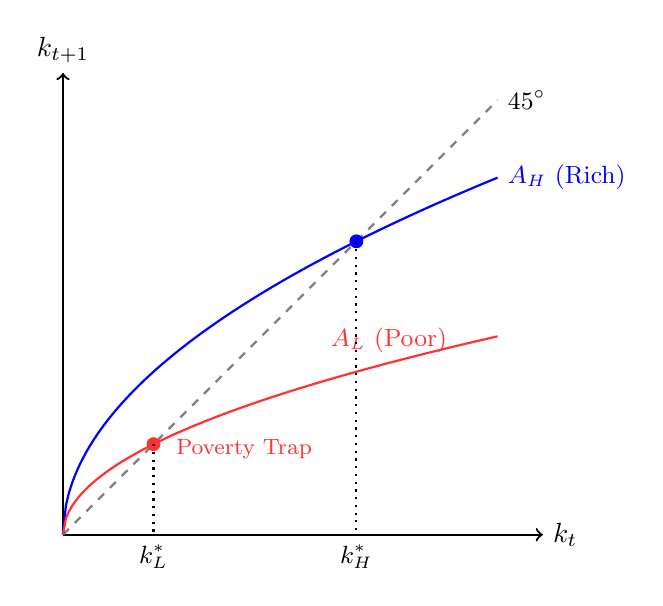
\begin{tikzpicture}[scale=1.15]
    % Axes
    \draw[->, thick] (0,0) -- (5.3,0) node[right] {$k_t$};
    \draw[->, thick] (0,0) -- (0,5.1) node[above] {$k_{t+1}$};

    % 45-degree line
    \draw[dashed, thick, gray] (0,0) -- (4.8,4.8)
        node[right, black, font=\small] {$45^\circ$};

    % High TFP: y = 1.8*sqrt(x), intersects 45-degree at x = 3.24
    \draw[thick, blue, domain=0:4.8, samples=150]
        plot (\x, {min(1.8*sqrt(\x), 4.8)})
        node[right, font=\small] {$A_H$ (Rich)};

    % Low TFP: y = 1.0*sqrt(x), intersects 45-degree at x = 1.0
    \draw[thick, red!80, domain=0:4.8, samples=150]
        plot (\x, {min(1.0*sqrt(\x), 4.8)});
    \node[red!80, font=\small] at (3.6, 2.15) {$A_L$ (Poor)};

    % Stable steady states
    \filldraw[blue] (3.24, 3.24) circle (2pt);
    \filldraw[red!80] (1.00, 1.00) circle (2pt);

    % Dotted projections to x-axis
    \draw[dotted, thick] (3.24, 3.24) -- (3.24, 0)
        node[below, font=\small] {$k_H^*$};
    \draw[dotted, thick] (1.00, 1.00) -- (1.00, 0)
        node[below, font=\small] {$k_L^*$};

    % Poverty trap annotation near low steady state
    \node[red!80, font=\footnotesize, align=left] at (2, 0.95)
        {Poverty Trap};
\end{tikzpicture}
\end{center}

Under this mechanism, the poverty trap is not a trap in the traditional sense of a basin of attraction with a tipping point. The poor economy is simply converging to a \textit{different}, structurally lower steady state. No matter how long we wait, it will not catch up to the rich economy---unless its structural fundamentals (institutions, technology, human capital) improve.

The key empirical implication is \textbf{conditional convergence}: controlling for the determinants of the steady state, economies with lower capital stocks grow faster. This is entirely consistent with the neoclassical model, and indeed the empirical literature on cross-country growth regressions finds considerably stronger support for conditional convergence than for the unconditional variety.

\rmk{The two mechanisms are conceptually distinct but not mutually exclusive. A country may face both non-convexities and structural disadvantages. Disentangling their relative importance is, as we shall see, an extraordinarily difficult empirical task.}

\section{Empirical Challenges: The Big Push}

\subsection{Concept and Motivation}

A natural policy response to the poverty trap---particularly if one believes Mechanism I---is the \textbf{Big Push}: a large-scale, coordinated injection of capital into a low-income economy with the aim of pushing $k_0$ above the tipping point $\hat{k}$ and into the basin of attraction of $k_H^*$. The idea was formalized by Murphy, Shleifer, and Vishny (1989) in a model of industrialization with increasing returns to scale, building on Rosenstein-Rodan's (1943) earlier insight that coordinated, large-scale investment could overcome the coordination failures preventing take-off.

The policy logic is compelling under Mechanism I: the required intervention may be large, but it need not be permanent. Once $k_0$ is pushed above $\hat{k}$, the economy accumulates on its own toward $k_H^*$, and the intervention can be withdrawn.

\subsection{The Identification Problem}

The empirical challenge is severe: \textit{regardless of whether a Big Push succeeds or fails, the outcome is consistent with both mechanisms.} This creates a fundamental identification problem.

\medskip

\noindent\textbf{Case 1: The push fails.} The economy receives a large capital infusion but eventually reverts to low income.

\begin{itemize}
    \item Under Mechanism I: the injection may have been substantial but still insufficient to push $k_0$ past $\hat{k}$. We do not know where $\hat{k}$ lies, and a failed push cannot tell us the economy received \textit{enough} capital to test whether the threshold exists.
    \item Under Mechanism II: capital alone cannot raise the steady state if TFP remains unchanged. The economy was always converging to a structurally low $k_L^*$, and the capital simply depreciated.
\end{itemize}
A failed push does not allow us to distinguish between the two explanations.

\medskip

\noindent\textbf{Case 2: The push succeeds.} The economy receives a large capital infusion and subsequently exhibits rapid, sustained growth.

\begin{itemize}
    \item Under Mechanism I: this is the predicted outcome---the economy crossed $\hat{k}$ and is now converging to $k_H^*$.
    \item Under Mechanism II: large-scale interventions rarely deliver capital alone. They typically come packaged with technology transfer, institutional reform, managerial expertise, and infrastructure investment---all of which raise $A_L$ toward $A_H$, shifting the entire law of motion upward. Under Mechanism II, the economy converges to a newly elevated $k^*$; the capital infusion was the vehicle, but the structural improvement was the cause.
\end{itemize}
A successful push does not cleanly identify Mechanism I as the correct explanation either.

\medskip

This identification problem is deep and not merely a matter of better data. The two mechanisms are, in many empirically relevant situations, \textit{observationally equivalent}: the same cross-country patterns of growth are consistent with either a world of multiple stable steady states or a world of heterogeneous but unique steady states. This is one of the central methodological difficulties in empirical development economics.

\subsection{Policy Implications of the Two Mechanisms}

Despite the identification challenge, the two mechanisms carry sharply different policy prescriptions.

Under Mechanism I, the key lever is \textit{crossing the threshold}. A targeted, temporary capital injection---if sufficiently large---can permanently transform a poor economy's trajectory. The intervention must be big, but it need not be sustained indefinitely; the economy's own internal dynamics carry it to $k_H^*$ once it is above $\hat{k}$.

Under Mechanism II, a capital injection alone is insufficient. The structural sources of low TFP---weak institutions, geographic barriers, low human capital, or technological backwardness---must be addressed directly. Capital without structural reform will simply depreciate, and the economy will return to $k_L^*$. Policy must target the fundamentals, not just the capital stock.

A plausible view is that both mechanisms operate simultaneously: poverty traps partly reflect non-convexities and partly reflect structural disadvantage, with the relative importance varying by country and historical context. This makes the design of effective development policy inherently difficult and context-dependent.

\rmkb[Development Economics and the Experimental Approach]{
    A strand of the development economics literature, closely associated with Esther Duflo and Abhijit Banerjee (Nobel Prize 2019), has attempted to make progress on these questions through \textbf{randomized controlled trials (RCTs)}. Rather than studying Big Push experiments at the national level---where identification is nearly impossible given the confounding of capital, technology, and institutions---this approach evaluates targeted interventions at the household or village level, aiming to isolate the causal effect of capital infusions on income and investment behavior.

    While greatly improving causal identification within their specific context, micro-level RCTs face their own important limitations. Interventions at small scales may fail to replicate the \textit{general equilibrium} complementarities, coordination effects, and agglomeration economies that lie at the heart of the Big Push mechanism. A village-level cash transfer is simply not the same as a national industrialization drive. The external validity of micro-level experiments for macro-level policy questions therefore remains an active and contentious area of debate.
}

\rmk{This chapter connects directly to the broader convergence debate. If Mechanism II is correct, convergence is conditional on structural fundamentals: economies with similar TFP levels converge to similar steady states, consistent with the neoclassical model and the empirical finding of conditional convergence. If Mechanism I is correct, convergence depends on initial conditions in a fundamentally more path-dependent way: history matters, and similar structural fundamentals may still give rise to different long-run outcomes depending on where the economy started relative to $\hat{k}$.}

